\documentclass[11pt,reqno]{amsart}
\usepackage{epsfig}
\usepackage{amsfonts}
\usepackage{graphicx}
\usepackage{amsmath}
\usepackage{amssymb}
%\usepackage{mathrsfs}
\setcounter{MaxMatrixCols}{10}
\hfuzz=12pt
\hbadness=5000
\vbadness=5000
\frenchspacing
\vfuzz=2pt
\input{epsf}
%\input{tcilatex}

\begin{document}

\title[Smooth Yield Curves For Euribor Estimation]{Bootstrapping the Illiquidity \\ \footnotesize{\emph{Post Credit Crunch Smooth Yield Curves Construction \\
For Market Coherent Forward Rates Estimation}}}

\author{Ferdinando M. Ametrano}
\address{Financial Engineering, Banca IMI, Piazzetta G. Dell'Amore 3, 20121
Milan Italy, ferdinando.ametrano(AT)bancaimi.com}

\author{Marco Bianchetti}
\address{Risk Management, Banca IntesaSanpaolo, Piazza G. Ferrari 10, 20121
Milan Italy, marco.bianchetti(AT)intesasanpaolo.com}

\thanks{JEL Classifications: E45, G13. \\ The authors acknowledges fruitful discussions with S. De Nuccio, R. Giura, C. Maffi, F. Mercurio, N. Moreni and the QuantLib community. The opinions expressed here are solely of the authors and do not represent in any way those of theirs employers.}

\date{Draft v. 0.4, Feb. 7th, 2008}

\keywords{liquidity, crisis, interest rates, yield curve, forward curve, discount curve, bootstrapping, pricing, hedging, interest rate derivatives, FRAs, Futures, swaps, basis swaps, QuantLib.}

\begin{abstract}
The large basis spreads observed on the interest rate market since the liquidity crisis of summer 2007 imply that different yield curves are required for market coherent estimation of forward rates with different tenors (e.g. Euribor 3 months, Euribor 6 months, etc.).
\\ In this paper we revise the methodology for bootstrapping interest rate yield curves from plain vanilla derivatives quoted on the market.
In particular we describe how to extract multiple yield curve term structures, each homogeneous in the underlying rate tenor, from non-homogeneous instruments such as deposits, Forward Rate Agreements, Futures, swaps, and basis swaps. The approach includes turn-of-year effects and is robust to deliver smooth yield curves and to ensure non-negative rates also in highly stressed market situations, characterized by crazy roller coaster shapes of the market quotations.
\\ The concrete EUR market case is analyzed in detail, using the open source QuantLib implementation of the proposed algorithms.
\end{abstract}

\maketitle

\section{\label{SecIntro}Introduction}
Pricing complex interest rate derivatives requires modeling the future dynamics of the yield curve term structure. Most of the literature assumes the existence of the \emph{current} yield curve as given, and its construction is often neglected as it is considered more an art than a science. Actually any yield curve term structure modeling approach will fail to produce good/reasonable prices if the current term structure is not correct.

Financial institutions, software houses and practitioners have developed various methodologies in order to extract the yield curve term structure from quoted prices of a finite number of liquid market instruments. \textquotedblleft Best-fit\textquotedblright\ algorithms assume a smooth functional form for the term structure and calibrate its parameters such that to minimize the repricing error of the chosen set of calibration instruments. For instance, the European Central Bank publishes yield curves on the basis of the Soderlind and Svensson (1997) model \cite{SodSwe97}, which is an extension of the Nelson-Siegel (1987) model (see e.g. refs. \cite{NelSie97}, \cite{Diament}, \cite{ChrDie07} and \cite{Cor08}). Such approach is popular due to the smoothness of the curve, calibration easiness, intuitive financial interpretation of functional form parameters (level, slope, curvature) and correspondence with principal component analysis. On the other side, the fit quality is typically not good enough for trading purposes in liquid markets.
\par
In practice \textquotedblleft exact-fit\textquotedblright\ algorithms are often preferred: they fix the yield curve on a time grid of $N$ points (pillars) in order to \emph{exactly} reprice $N$ pre-selected market instruments. The implementation of such algorithms is often incremental, extending the yield curve step-by-step with the increasing maturity of the ordered instruments, in a so called \textquotedblleft bootstrap\textquotedblright approach. Intermediate yield curve values are obtained by interpolation on the bootstrapping grid. Here different interpolation algorithms are available but little attention has been devoted in the literature to the fact that interpolation is often already used during bootstrapping, not just after that, and that the interaction between bootstrapping and interpolation can be subtle if not nasty (see e.g. \cite{HagWes06}, \cite{HagWes08}).

Whilst naive algorithms may fail to deal with market subtleties such as date conventions, the intra-day fixing of the first floating payment of a swap, the turn-of-year effect, the Futures convexity adjustment, etc., even very sophisticated algorithms used in a naive way may fail to estimate correct forward Euribor rates in difficult market conditions. Namely using just one single curve is not enough to account for forward Euribor rates of different tenor, such as 1, 3, 6, 12 months, because of the large basis swap spreads observed since the summer of 2007 in occasion of the so-called {\it subprime credit crunch crisis.}

The plan of the paper is as follows:
in section \ref{SecPricing} we review the traditional (old style) single curve market practice for pricing and hedging interest rate derivatives and the recent market evolution, triggered by the credit crunch crisis, towards a double-curve approach;
in section \ref{SecMath} we fix the notation and nomenclature;
in section \ref{SecBootstrapping} we describe the market instruments available for the bootstrap, detailing their peculiarities, and we introduce the multiple curves approach based on accurate instrument selection.
The next three following sections deal with issues crucial for smooth curve bootstrapping:
section \ref{SecTOY} shows how to estimate the turn-of-year effect and incorporate it as a jump in the yield curve bootstrapping;
section \ref{SecInterp} sets the record straight on sensitive interpolation choices;
section \ref{SecSynt} illustrates how to allocate the discount factor decrease in the underspecified first period in a way coherent with interpolated market FRAs.
Then, in section \ref{SecimplementationResults} we describe the numerical results delivered by the proposed framework, along with a quick overview of the corresponding open-source QuantLib implementation and of its Excel interface, able to bootstrap multiple yield curves in real-time for real-life needs.
Finally, in section \ref{SecPricing2curves} we take a look of the consequences of using different curves for calculating forward rates and discount factors on no arbitrage conditions and on pricing expression for interest rate derivatives.
Conclusions are collected in section \ref{SecConclusions}.

\section{\label{SecPricing}Pricing \& Hedging Interest Rate Derivatives}
One of the many consequences of the liquidity crisis started in the second half of 2007 has been a strong increase of the basis spreads quoted on the market between single-currency interest rate instruments, swaps in particular, characterized by different underlying rate tenors (e.g. Euribor3M\footnote{Euro Interbank Offered Rate, the rate at which euro interbank term deposits within the euro zone are offered by one prime bank to another prime bank (see e.g. www.euribor.org).}, Euribor6M, etc.), reflecting the increased liquidity risk and the corresponding preference of financial institutions for receiving payments with higher frequency (quarterly instead of semi-annualy, for instance).
\par
There are also other indicators of regime changes in the interest rate markets, such as the divergence between deposit (Euribor based) and OIS (Overnight Indexed Swaps, Eonia\footnote{Euro OverNight Index Average, the rate computed as a weighted average of all overnight rates corresponding to unsecured lending transactions in the euro-zone interbank market (see e.g. www.euribor.org).} based) rates with the same maturity, or between FRA (Forward Rate Agreement) contacts and the corresponding forward rates implied by consecutive deposits.
\par
The asymmetries cited above have also induced a sort of "segmentation" of the interest rate market into sub-areas, mainly corresponding to instruments with 1M, 3M, 6M, 12M underlying rate tenors, characterized, in principle, by different internal dynamics, liquidity and credit risk premia, reflecting the different views and interests of the market players. We stress that such new market situation is nothing else that a new equilibrium configuration determined by the pressure of the increased illiquidity force, that magnifies well known effects historically very small and traditionally neglected before the crisis (see also the discussion in refs. \cite{Mor08}, \cite{Mer09}).
\par
The evolution of the financial markets briefly described above has triggered a general reflection about the methodology used to price and hedge interest rate derivatives, namely those financial instruments whose price depends on the present value of future interest rate-linked cashflows.

\subsection{\label{SecSingleCurve}The Traditional Single Curve Approach}
The pre-crisis standard market practice (which does not automatically mean good practice) can be summarized in the following procedure (see e.g. refs. \cite{Ron00}, \cite{HagWes06}, \cite{And07} \cite{HagWes08}):

\begin{enumerate}
\item select \emph{one} finite set of the most convenient (e.g. liquid) vanilla interest rate instruments traded in real time on the market with increasing maturities; for instance, a very common choice in the EUR market is a combination of short-term EUR\ deposit, medium-term Futures on Euribor3M and medium-long-term swaps on Euribor6M;

\item build \emph{one} yield curve using the selected instruments plus a set of bootstrapping rules (e.g. pillars, priorities, interpolation, etc.);

\item compute \emph{on the same curve} forward rates, cashflows\footnote{within the present context of interest rate derivatives we focus in particular on forward rate dependent cashflows.}, discount factors and work out the prices by summing up the discounted cashflows;

\item compute the delta sensitivity and hedge the resulting delta risk using the suggested amounts (hedge ratios) of the \emph{same} set of vanillas.
\end{enumerate}

For instance, a 5.5Y maturity EUR floating swap leg on Euribor1M (not directly quoted on the market) is commonly priced using discount factors and forward rates calculated on the same depo-Futures-swap curve cited above. The corresponding delta sensitivity is calculated by shocking one by one the curve pillars and the resulting delta risk is hedged using the suggested amounts (hedge ratios)\ of 5Y and 6Y Euribor6M swaps\footnote{we refer here to the case of local yield curve bootstrapping methods, for which there are no sensitivity delocalization effect (see refs. \cite{HagWes06}, \cite{And07} \cite{HagWes08}).}.

We stress that this is a \emph{single-currency-single-curve approach}, in that a \emph{unique} curve is built and used to price and hedge any interest rate derivative on a given currency. Thinking in terms of more fundamental variables, e.g. the short rate, this is equivalent to assume that there exist a unique fundamental underlying short rate process able to model and explain the whole term structure of interest rates of any tenor.

It is also a \emph{relative pricing} approach, because both the price and the hedge of a derivative are calculated relatively to a set of vanillas quoted on the market. We notice also that the procedure is not strictly guaranteed to be arbitrage-free, because discount factors and forward rates obtained through interpolation are, in general, not necessarily consistent with the no arbitrage condition; in practice bid-ask spreads and transaction costs virtually hide any arbitrage possibility.

Finally, we stress that the first key point in the procedure above is much more a matter of art than of science, because there is not an unique financially sound choice of bootstrapping instruments and, in principle, none is better than the others.

The pricing \& hedging methodology described above can be extended, in principle, to more complicated cases, in particular when a model of the underlying interest rate evolution is used to calculate the future dynamic of the yield curve and the expected cashflows. The volatility and (eventually) correlation dependence carried by the model implies, in principle, the bootstrapping of a variance/covariance matrix (two or even three dimensional) and hedging the corresponding sensitivities (vega and rho) using volatility and correlation dependent vanilla market instruments. In practice just a small subset of such quotations is available on the market, and thus only some portions of the variance/covariance matrix can be extracted from the market. In this paper we will focus only on the basic matter of yield curves and forget the volatility/correlation dimensions.

\subsection{\label{SecMultiCurve}The New Multi Curve Approach}
Unfortunately, the pre-crisis approach outlined above is no longer consistent, at least in this simple formulation, with the present market configuration.

First, it does not take into account the market information carried by the basis swap spreads, now much larger than in the past and no longer negligible.

Second, it does not take into account that the interest rate market is segmentated into sub-areas corresponding to instruments with different underlying rate tenors, characterized, in principle, by \emph{different} dynamics (e.g. short rate processes). Thus, pricing and hedging an interest rate derivative on a single yield curve mixing different underlying rate tenors can lead to \textquotedblleft dirty\textquotedblright\ results, incorporating the different dynamics, and eventually the inconsistencies, of different market areas, making prices and hedge ratios less stable and more difficult to interpret. On the other side, the more the vanillas and the derivative share the same homogeneous underlying rate, the better should be the relative pricing and the hedging.

Third, by no arbitrage, discounting must be univocal: two identical future cashflows of whatever origin must display the \emph{same} present value; hence we need an unique discounting curve.

The market practice has thus evolved to take into account the new market informations cited above, that translate into the additional requirement of \emph{homogeneity}: as far as possible, interest rate derivatives with a given underlying rate tenor should be priced and hedged using vanilla interest rate market instruments with the \emph{same} underlying. We summarize here the following modified working procedure:

\begin{enumerate}
\item build \emph{one discounting curve} using the preferred procedure;

\item select \emph{multiple separated} sets of vanilla interest rate instruments traded in real time on the market with increasing maturities, each set \emph{homogeneous} in the underlying rate (typically with 1M, 3M, 6M, 12M tenors);
\item build \emph{multiple separated forwarding curves} using the selected instruments plus their bootstrapping rules;
\item compute \emph{on each forwarding curve} the forward rates and the corresponding cashflows relevant for pricing derivatives on the \emph{same} underlying;
\item compute the corresponding discount factors using the discounting curve and work out prices by summing up the discounted cashflows;
\item compute the delta sensitivity and hedge the resulting delta risk using the suggested amounts (hedge ratios) of the \emph{corresponding} set of vanillas.
\end{enumerate}

For instance, the 5.5Y floating swap leg cited in the previous section should be priced using Euribor1M forward rates calculated on an \textquotedblleft pure\textquotedblright\ 1M forwarding curve, bootstrapped only on Euribor1M vanillas, plus discount factors calculated on the discounting curve. The corresponding delta sensitivity should be calculated by shocking one by one the pillars of both yield curves, and the resulting delta risk hedged using the suggested amounts (hedge ratios)\ of 5Y and 6Y Euribor1M swaps plus the suggested amounts of 5Y and 6Y instruments from the discounting curve.

The improved approach described above is more consistent with the present market situation, but - there is no free lunch - it does demand much more additional efforts. First, the discounting curve clearly plays a special and fundamental role, and must be built with particular care. This \textquotedblleft pre-crisis\textquotedblright\ obvious step has become, in the present market situation, a very subtle and controversial point, that would require a whole paper in itself. In fact, while the forwarding curves construction is driven by the underlying rate tenor homogeneity principle, for which there is (now) a general market consensus, there is no longer general consensus for the discounting curve construction. At least two different practices can be encountered on the market: a) the old
\textquotedblleft pre-crisis\textquotedblright\ approach (e.g. the depo, Futures and swap curve cited before), that can be justified with the principle of maximum liquidity (plus a little of inertia), and b) the Eonia curve, justified with no risky or collateralized counterparties, and by increasing liquidity (see e.g. the discussion in ref. \cite{Mad08}).
Second, building multiple curves requires multiple quotations: much more interest rate bootstrapping instruments must be considered (deposits, Futures, swaps, basis swaps, FRAs, etc.), which are available on the market with different degrees of liquidity and can display transitory inconsistencies.
Third, non trivial interpolation algorithms are crucial to produce smooth forward curves (see e.g. refs. \cite{HagWes08}, \cite{And07}).
Fourth, multiple bootstrapping instruments implies multiple sensitivities, so hedging becomes more complicated. Last but not least, pricing libraries, platforms, reports, etc. must be extended, configured, tested and released to manage multiple and separated yield curves for forwarding and discounting, not a trivial task for quants, developers and IT\ people.


\section{\label{SecMath}Fixing Notation and Nomenclature}
In this section we fix notation and nomenclature for our multi-curve environment, inspired by refs. \cite{Bia09},\cite{Mer09}. Following the discussion of section \ref{SecPricing} (see also refs. \cite{Bia09}, \cite{Mer09}), we start by postulating the existence of $N$ distinct interest rate markets, denoted by $M_{x}$. The index $x$ will take the values associated to the corresponding yield curves, e.g. $x=\left\{d,1M,3M,6M,12M\right\}$, where $d$ stands for discounting and $1M,3M,6M,12M$ stand for the underlying rate tenors. The $N$ markets $M_{x}$ are characterized by the same currency and by distinct bank accounts $B_{x}$ and yield curves $\mathcal{C}_{x}$ in the form of a continuous term structure of discount factors,
\begin{equation}
\mathcal{C}_{x}=\left\{ T\longrightarrow P_{x}\left( t_{0},T\right) ,T\geq t_{0}\right\} ,
\end{equation}
where $t_{0}$\ is the reference date of the curve, e.g. today, or settlement date (which in the EUR money market is two business days after today, according to the TARGET\footnote{Trans-european Automated Real-time Gross settlement Express Transfer.} holiday calendar) and $P_{x}\left(t,T\right)$ denotes the price at time $t\geq t_{0}$ of the \textit{x}-zero coupon bond for maturity $T$, such that $P_{x}\left( T,T\right) =1$.

Time intervals between couples of dates $\left[T_{1},T_{2}\right]$ are measured in each market $M_{x}$ as year fractions with a given day count convention $dc_x$, $\tau\left(T_{1},T_{2};dc_x\right)$.
In particular, the year fraction associated to discount factors must be monotonically increasing with increasing time intervals (non increasing convention would lead to spurious null forward rates), and additive, such that
\begin{equation}
\tau\left(T_{1},T_{2};dc_x\right) + \tau\left(T_{2},T_{3};dc_x\right)
= \tau\left(T_{1},T_{3};dc_x\right).
\end{equation}
The day count convention satisfying the above conditions that will be used in this paper (for any market $M_x$) is the common \emph{Actual/365 (Fixed)} \cite{ISDA}, such that:
\begin{equation}
\tau_{\mathcal{C}}\left(T_{1},T_{2}\right)
:= \tau\left[T_{1},T_{2};actual/365 (Fixed)\right]
= \frac{T_2-T_1}{365}.
\end{equation}
\\
Since the discount factor curve is observed to be exponentially decreasing, as expected when the interest rate compounding is made so frequent to be practically continuous, the yield curve is usually described through an exponential transformation, i.e. by continuously compounded zero coupon rates $z_x(t_0,T)$ or instantaneous forward rates\footnote{par rates could be used too; we do not use them here as they are not frequently used and would not provide additional benefit anyway.} $f_x(t)$ such that
\begin{equation}
P_x(t_0,T)
= \exp\left[-z_x\left(t_0,T\right)\tau_{\mathcal{C}}\left(t_0,T\right)\right]
= \exp\left[-\int_{t_0}^{T}f_x\left(u\right)du\right],
\label{eqn:relationship}
\end{equation}
or, using the equivalent $\log$ notation,
\begin{equation}
\log P_x(t_0,T)
= -z_x\left(t_0,T\right)\tau_{\mathcal{C}}\left(t_0,T\right)
= -\int_{t_0}^{T}f_x\left(u\right)du.
\label{eqn:logrelationship}
\end{equation}
From these relationships it is immediate to observe that:
\begin{itemize}
\item the starting point of the discount curve is $P_x(t_0,t_0)=1$ by construction, while $z_x\left(t_0,t_0\right) $ and $f_x\left(t_0\right)$ are less significant values, being just limits for shrinking $T\rightarrow t_0$. Therefore it makes sense for a discount factor grid to add the $\left(t_0,P_x=1\right)$ extra point, while an equivalent choice for zero or forward rates is to some extent arbitrary and as such must be handled with care;
\item $z_x\left(t_0,T\right)$ is the average of $f_x\left(u\right)$ over $\left[t_0,T\right]$;
\item the instantaneous forward rate curve $f_x\left(t\right)$ is the most severe indicator of yield curve smoothness, since anything else is obtained through its integration (therefore being smoother by construction).
\end{itemize}
Besides when rates are non-negative (as it is in all western markets and in the EUR market we consider in this paper):
\begin{itemize}
\item ($\log $) $P(t_0,T)$ is a monotone non-increasing function of $T$. Therefore it would make sense to interpolate on a (log-)discount grid with an algorithm that ensures monotonicity;
\item $P\left(t_0,T\right)>0\quad\forall\,T>t_0$.
\end{itemize}
\par
The usual no arbitrage relation among discount factors holds in each market $M_{x}$,
\begin{equation}
P_{x}\left(t,T_{2}\right)
= P_{x}\left(t,T_{1}\right) \times P_{x}\left(t,T_{1},T_{2}\right),
\quad\forall\, t_0 \leq t \leq T_{1}<T_{2},
\label{eqn:NoArbitrage}
\end{equation}
where $P_{x}\left(t,T_{1},T_{2}\right) $ denotes the forward discount factor from time $T_{2}$ to time $T_{1}$, prevailing at any time $t\geq t_0$. The financial meaning of expression (\ref{eqn:NoArbitrage}) is that, in each market $M_{x}$, given a cashflow of one unit of currency at time $T_{2}$, its corresponding value at time $t<T_{2}$ must be the same both if we discount in one single step from $T_{2}$ to $t$, using the discount factor $P_{x}\left(t,T_{2}\right)$, and if we discount in two steps, first from $T_{2}$ to $T_{1}$, using the forward discount $P_{x}\left(t,T_{1},T_{2}\right)$ and then from $T_{1}$ to $t$, using $P_{x}\left(t,T_{1}\right)$. Denoting with $F_{x}\left(t;T_{1},T_{2}\right)$ the simple compounded forward rate associated to $P_{x}\left(t,T_{1},T_{2}\right)$, resetting at time $T_{1}$ and covering the time interval $\left[T_{1},T_{2}\right]$ with \emph{actual/360} day count convention, we have
\begin{equation}
P_{x}\left(t,T_{1},T_{2}\right)
= \frac{P_{x}\left(t,T_{2}\right)}{P_{x}\left(t,T_{1}\right)}
= \frac{1}{1+F_{x}\left(t;T_{1},T_{2}\right)\tau_F\left(T_{1},T_{2}\right) },
\label{eqn:FwdRate}
\end{equation}
where we have defined
\begin{equation}
\tau_F\left(T_{1},T_{2}\right) := \tau\left(T_{1},T_{2};actual/360\right).
\label{eqn:yfFRA}
\end{equation}
From eq. (\ref{eqn:NoArbitrage}) we obtain the familiar no arbitrage expression
\begin{eqnarray}
F_{x}\left(t;T_{1},T_{2}\right)
&=& \frac{1}{\tau_F\left(T_{1},T_{2}\right)}\left[\frac{1}{P_{x}\left(t,T_{1},T_{2}\right) }-1\right]   \notag \\
&=& \frac{P_{x}\left(t,T_{1}\right) - P_{x}\left(t,T_{2}\right)}{\tau_F\left(T_{1},T_{2}\right) P_{x}\left(t,T_{2}\right)}.
\label{eqn:FwdRate}
\end{eqnarray}
\par
Regarding swap rates, given two increasing dates vectors
$\mathbf{T=}\left\{T_{0},...,T_{n}\right\}$,
$\mathbf{S=}\left\{S_{0},...,S_{m}\right\}$, $T_{0}=S_{0}\geq t_0$, and an interest rate swap with a floating leg paying at times $T_{i}$, $i=1,..,n$, the Euribor rate with tenor
$\left[T_{i-1},T_{i}\right]$ fixed at time $T_{i-1}$, plus a fixed leg paying a fixed rate at times $S_{j}$, $j=1,..,m$, the corresponding fair swap rate on curve $\mathcal{C}_{x}$ with \emph{30/360 (Bond Basis)} day count convention is given by
\begin{eqnarray}
S_{x}\left(t,\mathbf{T},\mathbf{S}\right)
&=& \frac{\sum\limits_{i=1}^{n}P_{x}\left(t,T_{i}\right) \tau_F\left(T_{i-1},T_{i}\right) F_{x}\left(t;T_{i-1},T_{i}\right)}{A_{x}\left(t,\mathbf{S}\right)} \notag \\
&=& \frac{P_{x}\left(t,T_0\right) - P_{x}\left(t,T_n\right)}{A_{x}\left(t,\mathbf{S}\right)}
,\quad t_0\leq t\leq T_{0}
\label{eqn:SwapRateFwd}
\end{eqnarray}
where
\begin{equation}
A_{x}\left(t,\mathbf{S}\right)
= \sum\limits_{j=1}^{m}P_{f}\left(t,S_{j}\right) \tau_S\left(S_{j-1},S_{j}\right)
\end{equation}
is the annuity on curve $\mathcal{C}_{x}$ and we have defined
\begin{equation}
\tau_S\left(T_{i-1},T_{i}\right)
:= \tau\left[T_{1},T_{2};30/360\,(Bond Basis)\right].
\end{equation}

\section{\label{SecBootstrapping}Bootstrapping Euribor Curves}
In this section we first review and criticize the standard pre-crisis bootstrapping methodology for interbank Euribor curves, then we examine in detail all the market instruments used in the new multi curve framework.

\subsection{Single Curve Bootstrapping}
A summary of standard pre-crisis bootstrapping methodology is given in common textbooks as, for instance, \cite{Hul08} and \cite{Reb1998}.
Different kinds of instruments can be selected for bootstrapping an yield curve term structure, and whilst they roughly cover different maturities, they overlap in significant areas. Therefore it is usually impossible to include all the available instruments, and the subset of the mostly non-overlapping instruments is selected, with preference given to more liquid ones with a tighter bid/ask spread. The mispricing level of the excluded instruments must thus be monitored as safety check (or cheap-rich analysis).
\par
The so-called interbank Euribor curve was usually bootstrapped from the following market instruments:
\begin{itemize}
\item Deposit contracts, covering the period from today up to 1Y;
\item Forward Rate Agreement contracts (FRAs), covering cover the period from 1M up to 2Y;
\item Short term interest rate Futures contracts, covering the period from spot/3M (depending on the current calendar date) up to 2Y and more;
\item Swap contracts, covering the period from 1Y up to 60Y.
\end{itemize}
The instrument set above overlaps (by maturity) at the deposit/Futures and Futures/swaps borders. Overlapping instruments are selected according to the principle of maximum liquidity: Futures with short expiries are the most liquid, so they have priority higher than deposits and short term swaps. For longer expiries Futures are not as liquid, so swaps are used.

\subsection{Multi Curve Bootstrapping}
[NOTA: da rivedere prima parte di testo]

As mentioned in section \ref{SecPricing}, in the present post credit crunch market situation, distinct interest rate market segments $M_x$, relative to different Euribor rate tenors, are characterized by different internal dynamics, liquidity and credit risk premia, reflecting the different views and interests of the market players.
Such more complex market mechanic generates the following features:
\begin{itemize}
\item similar market instruments insisting on different underlyings, for instance FRAs or swaps on Euribor3M and Euribor6M, may display very different price levels;
\item similar market instruments may display very different relative liquidities;
\item even small idiosyncracies, asynchronies and inconsistencies in market quotations may result in erratic forward rates.
\end{itemize}
Hence, the first step for multiple yield curve construction is a very careful selection of the corresponding multiple sets of bootstrapping instruments. In the following subsections we examine these instruments in detail. We refer to the market quotes observed as of 23th Jan. 2009.

\subsubsection{\label{SecDepo}Deposits}
Interest rate deposit contracts (depos) quoted in the EUR market start at spot date (two working days after today, according to the TARGET holiday calendar) and span the length indicated by their maturity. Exceptions are the {\it over-night} (ON) and {\it tomorrow-next} (TN) one-day deposits, which start today and tomorrow, respectively, and cover (without overlapping) the interval between today and spot date.
The maturity date of deposits shorter than one month obeys the {\it Following} convention; for longer deposits the convention is {\it Modified Following}. For the latters the {\it end-of-month} convention is also respected: if the start date is the last working day in a given month, the end date must be the last working date of the ending month too.
\begin{table}[btp]
\label{tab:deposits}
\begin{tabular}{cccccccc}
Tenor & Rate & Settlement & Business       & End of & Start & End  & Year \\
      &      &            & day convention & month   & Date  & Date & Fraction \\
ON & 1.0000\% & today & Following &  &  \\
TN & 1.0000\% & tomorrow & Following &  &  \\
SN & 1.0000\% & spot & Following &  &  \\
SW & 1.0000\% & spot & Following &  &  \\
1W & 1.0000\% & spot & Following &  &  \\
2W & 1.0000\% & spot & Following &  &  \\
3W & 1.0000\% & spot & Following &  &  \\
1M & 1.0000\% & spot & Modified Following &  &  \\
2M & 1.0000\% & spot & Modified Following &  &  \\
3M & 1.0000\% & spot & Modified Following &  &  \\
4M & 1.0000\% & spot & Modified Following &  &  \\
5M & 1.0000\% & spot & Modified Following &  &  \\
6M & 1.0000\% & spot & Modified Following &  &  \\
9M & 1.0000\% & spot & Modified Following &  &  \\
12M & 1.0000\% & spot & Modified Following &  &  \\
&  &  &  &  &
\end{tabular}%
\caption{Depo strip. Source: Reuters page XXX (NOTA: verificare pagina), 23rd Jan. 2009.}
\end{table}
\par
In table \ref{tab:deposits} we report the depo strip quoted in Reuters page XXX (NOTA: verificare pagina).
If $R^{depo}_x\left(t_0,T_i\right)$ is the quoted rate associated to the i-th deposit with maturity $T_i$ and underlying rate tenor $x=T_i - t_0$ months, we have that the implied discount factor at time $T_i$ is given by\footnote{here we keep the subscript $x$ explicit also to be consistent with eq. (\ref{eqn:FRA}).}
\begin{equation}
P_x(t_0,T_i) = \frac{1}{1 + R^{depo}_x\left(t_0,T_i\right)\tau_F\left(t_0,T_i\right)},\quad t_0<T_i,
\label{eqn:deposit}
\end{equation}
where $\tau_F$ is given by eq. (\ref{eqn:yfFRA}). Notice that the reference date $t_0$ is different for ON, TN and other depos
\par
Market deposits can be selected as bootstrapping instruments for the construction of the short term structure section of the yield curves. Notice that each depo admits a different underlying rate tenor, corresponding to its maturity. Hence each depo can be selected, in principle, for the construction of a single curve. We will discuss this point in section \ref{SecSynt}.

\subsubsection{\label{SecFRA}Forward Rate Agreements (FRAs)}
FRA contacts are forward starting deposits. For instance the 3x9 FRA is a six months deposit starting three months forward. In the EUR market the forward start date (i.e. the start date of the forward depo) is calculated with the same convention used for the end date of deposits, so FRAs do concatenate exactly, e.g. the 6x9 FRA starts when the preceding 3x6 FRA ends. The underlying forward rate fixes two working days before the forward start date (NOTA: VERIFICARE).
In table \ref{tab:deposits} we report the three FRA strips on 3M, 6M, and 12M Euribor rate quoted in Reuters page XXX (NOTA: verificare ).
\begin{table}[btp]
\label{tab:FRA}
\begin{tabular}{cccccc}
Type & Rate & Start Date & End Date &  &  \\
1x4 & 1.0000\% &  &  &  &  \\
2x5 & 1.0000\% &  &  &  &  \\
3x6 & 1.0000\% &  &  &  &  \\
4x7 & 1.0000\% &  &  &  &  \\
5x8 & 1.0000\% &  &  &  &  \\
6x9 & 1.0000\% &  &  &  &  \\
9x12 & 1.0000\% &  &  &  &  \\
1x7 & 1.0000\% &  &  &  &  \\
2x8 & 1.0000\% &  &  &  &  \\
3x9 & 1.0000\% &  &  &  &  \\
4x10 & 1.0000\% &  &  &  &  \\
5x11 & 1.0000\% &  &  &  &  \\
6x12 & 1.0000\% &  &  &  &  \\
12x18 & 1.0000\% &  &  &  &  \\
18x24 & 1.0000\% &  &  &  &  \\
12x24 & 1.0000\% &  &  &  &  \\
&  &  &  &  &
\end{tabular}%
\caption{FRA strips on Euribor3M, Euribor6M, and Euribor12M. Source: Reuters page XXX (NOTA: verificare pagina), 23rd Jan. 2009.}
\end{table}
If $F_{x}\left(t;T_{i-1},T_{i}\right)$ is the i-th Euribor forward rate resetting at time $T_{i-1}$ with tenor $x=T_{i}-T_{i-1}$ months associated to the i-th FRA with maturity $T_i$, we have that the implied discount factor is obtained by eq. (\ref{eqn:FwdRate}) as
\begin{equation}
P_x\left(t_0,T_i\right) = \frac{P_x\left(t_0,T_{i-1}\right)}{1+F_{x}\left(t_0;T_{i-1},T_{i}\right)\tau_F\left(T_{i-1},T_{i}\right) },\quad t_0<T_{i-1}<T_i,
\label{eqn:FRA}
\end{equation}
where $\tau_F$ is given by eq. (\ref{eqn:yfFRA}). We observe that FRAs collapse to depos for shrinking $T_{i-1}-t_0$
\begin{equation}
\lim_{T_{i-1} \to t_0}F_{x}\left(t_0;T_{i-1},T_{i}\right) = R^{depo}_x\left(t_0,T_i\right),
\end{equation}
hence eq. (\ref{eqn:FRA}) reduces to eq. (\ref{eqn:deposit})
\par
Market FRAs provide direct empirical evidence that a single curve cannot be used to estimate forward rates with different tenors. We can observe in \ref{tab:FRA} that, for instance, the level of the 1x4 FRA3M (spanning from March 3rd to June 3rd, $\tau_{F,3M} = 0.2555$) was $1.888\%$, the level of 4x7 FRA3M (spanning from June 3rd to September 3rd, $\tau_{F,3M} = 0.2555$) was $1.721\%$. If one would compound these two rates to imply the level of the 1x7 FRA6M (spanning from March 3rd to September 3rd, $\tau_{F,6M} = 0.5111$) would obtain
\begin{equation}
\frac{
    \left(1 + 0.01888 \times 0.255\right) \left(1 + 0.01721 \times 0.255\right) - 1.0}
    {0.5111 }
    = 1.809\%,
\label{eqn:FRAarbitrage}
\end{equation}
while the market rate for the $1x7$ was $2.008\%$, twenty basis point larger. As discussed in section \ref{SecPricing}, the difference is the liquidity/default risk premium seen by the market in post credit crunch times. [NOTA: aggiornare questi dati al 23 gennaio 2009]
\par
Market FRAs on $x$-tenor Euribor can be selected, together with the corresponding depos, as bootstrapping instruments for the construction of short term structure section of the yield curve with tenor $x$.

\subsubsection{\label{SecFutures}Futures}
\begin{table}[btp]
\label{tab:Futures}
\begin{tabular}{cccccc}
IMM  & Price & Convexity  & Forward & IMM  & End  \\
code &       & adjustment & Rate    & Date & Date \\
H8 & 97.34\% & 0.01\% & 3.65\% &  &  \\
H8 & 97.34\% & 0.01\% & 3.65\% &  &  \\
H8 & 97.34\% & 0.01\% & 3.65\% &  &  \\
H8 & 97.34\% & 0.01\% & 3.65\% &  &  \\
H8 & 97.34\% & 0.01\% & 3.65\% &  &  \\
H8 & 97.34\% & 0.01\% & 3.65\% &  &  \\
H8 & 97.34\% & 0.01\% & 3.65\% &  &  \\
H8 & 97.34\% & 0.01\% & 3.65\% &  &  \\
H8 & 97.34\% & 0.01\% & 3.65\% &  &  \\
H8 & 97.34\% & 0.01\% & 3.65\% &  &  \\
H8 & 97.34\% & 0.01\% & 3.65\% &  &  \\
H8 & 97.34\% & 0.01\% & 3.65\% &  &  \\
H8 & 97.34\% & 0.01\% & 3.65\% &  &  \\
H8 & 97.34\% & 0.01\% & 3.65\% &  &  \\
H8 & 97.34\% & 0.01\% & 3.65\% &  &  \\
H8 & 97.34\% & 0.01\% & 3.65\% &  &  \\
H8 & 97.34\% & 0.01\% & 3.65\% &  &  \\
H8 & 97.34\% & 0.01\% & 3.65\% &  &  \\
&  &  &  &  &
\end{tabular}%
\caption{Futures on 3M deposit}
\end{table}
Interest Rate Futures are the exchange-traded contracts equivalent to the over-the-counter FRAs. They are quoted in terms of prices instead of rates, the relation being
\begin{equation}
P^{Fut}_x\left(t_0,T_{i-1},T_i\right) = 100 - R^{Fut}_x\left(t_0,T_{i-1},T_i\right),
\label{eqn:futurepricerate}
\end{equation}
and admit the $x$-months Euribor rate as underlying.
\par
While FRAs have the advantage of being more customizable, Futures are highly standardized: in the EUR market they fix the third Wednesday of the maturity month; the last trading day is the preceding Monday (because of the two days of settlement); the most common contracts (so called IMM\footnote{International Money Market of the Chicago Mercantile Exchange.} Futures) insist on Euribor3M [NOTA: E BASTA ? VERIFICARE] and expire every March, June, September and December (IMM dates). There are also so called {\it serial} contracts expiring in the upcoming months not covered by the quarterly Futures. Maturities extend up to 5 years {NOTA: VERIFICARE}. Any profit and loss is regulated through daily marking to market (so called margining process), thus reducing the credit risk.
Such standard characteristics reduce the transaction costs and imply a very high liquidity. The first {\it front} contract is the most liquid interest rate instrument, with longer expiry contracts having very good liquidity up to the 8th-12th contract. Also the first serial contact is quite liquid, especially when its expiration is before the front contract.
\par
Because of their marking to market mechanism Futures do not have the same payoff of FRAs: an investor long a Futures contract will have a loss when the Futures price decrease but will finance such loss at lower rate (see \ref{eqn:futurepricerate}); viceversa when the Futures price increase the profit will be reinvested at higher rate [NOTA: VERIFICARE]. This means that the volatility of the forward rates and their correlation to the spot rates have to be accounted for, hence a {\it convexity adjustment} is needed to convert the rate $R^{Fut}_x$ implied in the Futures price to its corresponding forward rate $F_x$,
\begin{equation}
F_x\left(t_0,T_{i-1},T_i\right) = R^{Fut}_x\left(t_0,T_{i-1},T_i\right)-C_x\left(t_0,T_{i-1},T_i,\sigma_i,\rho_i\right),
\label{eqn:fwdfromfutureprice}
\end{equation}
While different approaches are available in literature (see e.g. refs. \cite{Jac05}, \cite{PitRen06}, \cite{Vaillant}), a practitioner reference recipe to estimate the convexity adjustment is due to  XXX and YYY, using a simple Hull \& White model \cite{HulWhi1990}. Their approach it's used in \ref{tab:Futures} to calculate adjustments using
$\sigma = 0.0$ and $\mu = 0.0$ [NOTA: VERIFICARE].
\par
Market Futures on $x$-tenor Euribor can be selected as bootstrapping instruments for the construction of short-medium term structure section of the yield curve with tenor $x$.
Notice that Futures contracts have expiration dates gradually shrinking to zero and as such they generate rolling pillars that periodically jumps and overlap the fixed depo and FRA pillars. Hence some {\emph priority} rule must be used to decide which instrument must be excluded from the bootstrapping procedure.

\subsubsection{\label{SecSwap}Swaps}
[NOTA: da rivedere (Marco)]
\begin{table}[tbp]
\label{tab:swaps6M}
\begin{tabular}{cc}
Tenor & Rate \\
2Y  & 3.34\% \\
3Y  & 3.34\% \\
4Y  & 3.34\% \\
5Y  & 3.34\% \\
6Y  & 3.34\% \\
7Y  & 3.34\% \\
8Y  & 3.34\% \\
9Y  & 3.34\% \\
10Y & 3.34\% \\
11Y & 3.34\% \\
12Y & 3.34\% \\
15Y & 3.34\% \\
20Y & 3.34\% \\
25Y & 3.34\% \\
30Y & 3.34\% \\
40Y & 3.34\% \\
50Y & 3.34\% \\
60Y & 3.34\% \\
&
\end{tabular}%
\caption{Fixed rate vs 6M Euribor swaps}
\end{table}

\begin{table}[tbp]
\label{tab:swaps3M}
\begin{tabular}{cc}
Tenor & Rate \\
12M & 3.34\% \\
15M & 3.34\% \\
18M & 3.34\% \\
21M & 3.34\% \\
&
\end{tabular}%
\caption{Fixed rate vs 3M Euribor swaps}
\end{table}

\begin{table}[tbp]
\label{tab:swapsIMM}
\begin{tabular}{cc}
Type & Rate \\
MAR/MAR & 3.34\% \\
JUN/JUN & 3.34\% \\
SEP/SEP & 3.34\% \\
MAR/MAR 2Y & 3.34\% \\
MAR/MAR 3Y & 3.34\% \\
&
\end{tabular}%
\caption{IMM dated fixed rate vs 3M Euribor swaps}
\end{table}

A vanilla swap is an over-the-counter contract in which two counterparties agree to exchange annual fixed rate cash flows against six (or three) month floating rate cash flows indexed to six (or three) month Euribor. These streams are called the legs of the swap. The floating leg can be regarded as a portfolio of forward contracts.

Assuming $P(0)=1$, from equation \ref{eqn:swaprate} one obtains:
\begin{equation}
P(\tau_T) = \frac
    {1 - S \sum_1^{T-1} \delta_j P(\tau_j)}
    {1+S \delta_T}
\label{eqn:discfromswaprate}
\end{equation}

The left side of equation \ref{eqn:swaprate} actually arise from the reduction of the telescopic sum of discounted floating leg cashflows; assuming semiannual floating payments at $t_i$ with $\alpha_i=daycount_{act/360}(t_{i-1},t_i) $ the floating leg present value is
\begin{equation}
\sum_1^{2T} L(t_{i-1},t_i) \alpha_i P(t_i)
\label{eqn:discfloatlegcf}
\end{equation}
using \ref{eqn:Euriborrate}

\begin{equation}
\sum_1^{2T} \frac{P(t_{i-1}) / P(t_i) - 1}{alpha_i} \alpha_i P(t_i)
\end{equation}

and simplifying:

\begin{equation}
P(0)-P(t_T)
\end{equation}

Anyway at XX Frankfurt time the first Euribor rate is fixed at level $E$, so equation \ref{eqn:swaprate} becomes
\begin{equation}
E \alpha_1 P(t_1) + P(t_1) - P(t_0+T) = S \sum_1^T \tau_j P(t_j)
\label{eqn:swapratewithfixingeffect}
\end{equation}


liquid swaps and interpolated ones


\subsubsection{\label{SecBasis}Basis Swaps}
TBD
\begin{table}[tbp]
\label{tab:basisSwaps}
\begin{tabular}{cc}
Type & Rate \\
MAR/MAR & 3.34\% \\
JUN/JUN & 3.34\% \\
SEP/SEP & 3.34\% \\
MAR/MAR 2Y & 3.34\% \\
MAR/MAR 3Y & 3.34\% \\
&
\end{tabular}%
\caption{Basis swaps}
\end{table}


\section{\label{SecTOY}The Turn-of-Year Effect}
TBD


\section{\label{SecInterp}The Role of Interpolation}
The interpolation we choose for the given parametrization determines how reasonable the yield curve will be. For instance, linear interpolation of the discount factors is an obvious but extremely poor choice. Linear interpolation of zero rates or log-discounts are popular choices leading to stable and fast bootstrapping procedures. Unfortunately they produce discontinuous forward rates, with a sagsaw or piecewise-constant shape.

flat extrapolation out to infinity.

well-documented problems with spurious inflection points, excessive convexity, and lack of locality in the effects of input price perturbations. Andersen \cite{And07} addresses these issues through the use of shape-preserving splines from the class of generalized tension splines.

swap selection

citare Hyman \cite{Hym1983}, \cite{HagWes06}, \cite{HagWes08}).


TBD: mostrare casi di cattiva interpolazione, ad es. linear on zero rates


\section{\label{SecSynt}Synthetic Instruments}
TBD:
problema dello scodamento. e sua soluzione tramite synthetic depos


\section{\label{SecimplementationResults}Implementation and Numerical Results}
\subsection{Implementation}
The results discussed above have been obtained by the authors using the QuantLib framework. The object oriented C++ QuantLib library \cite{QuantLib} offers tools for advanced modeling and practical implementation, with features such as market conventions, yield curve models, solvers, PDEs, (Quasi)\ Monte Carlo, exotic options, VAR, etc. The QuantLibAddin \cite{QuantLibAddin} and QuantLibXL \cite{QuantLibXL} projects use the ObjectHandler in-memory repository \cite{ObjectHandler} to export the QuantLib objects (classes) and analytic (methods) to a variety of end-user platforms including Excel and Calc. The full implementation of the work described before, comprehensive of C++ code and Excel workbooks, is open source. In particular...
[\emph{TBD: ampliare questo punto descrivendo meglio che cosa \`{e} effettivamente implementato e disponibile ?\ }]. Anyone interested in the topic is invited to post to the QuantLib community any comment or suggestion to improve the job.

\subsection{Numerical Results (TBD)}
Tests of repricing \ (grafici di repricing degli stessi strumenti sulle 4
curve con breve commento)

cap/floor parity

\begin{figure}[tbp]
\centering
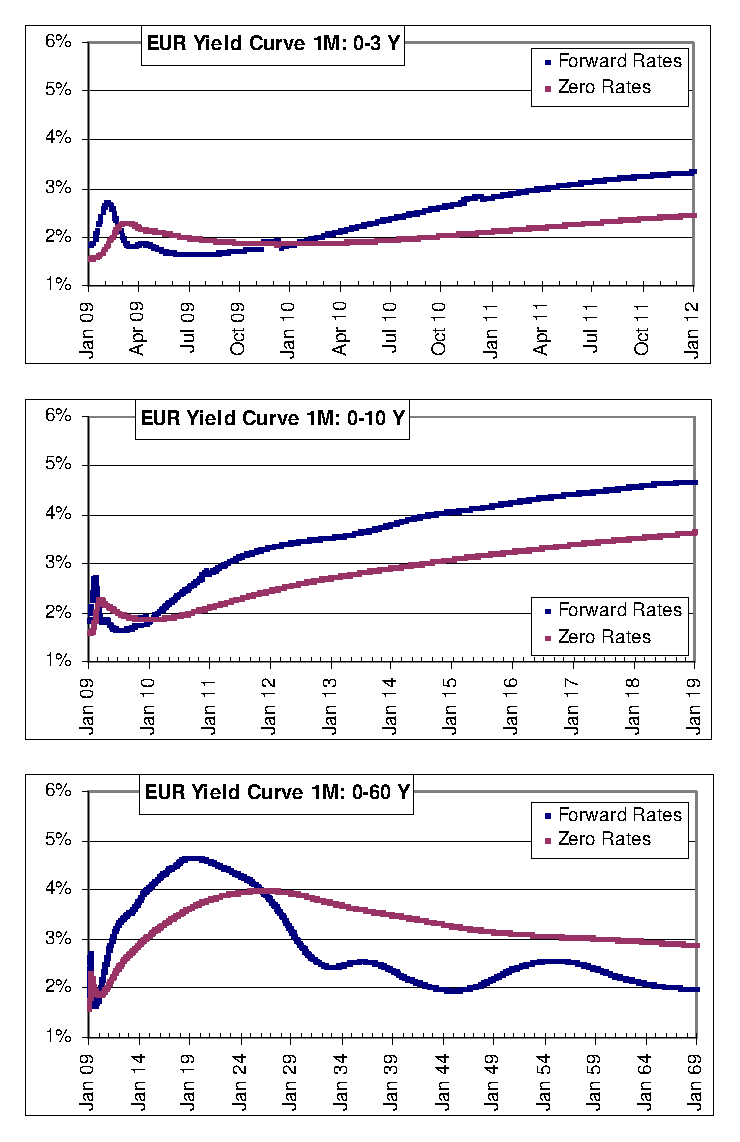
\includegraphics[scale=0.9]{./FigYC1M}
\caption{Yield curve on Euribor1M. Brown line: zero curve, plotted with zero rates $Z_{f}^{I_{1M}}\left(t_{0},t_{0}+t,\text{\textit{act/365}}\right)$, $t$ daily sampled and settlement date $t_{0}=$ Jan. 27th, 2009. Blu line: forward curve $\mathcal{C}_{f}^{I_{1M}}$, plotted with 1M-tenor forward rates $F\left( t_{0};t,t+1M,\text{\textit{act/360}}\right) $. Upper panel: short term structure up to 3 years; middle panel: medium term structure up to 10 years; lower panel: long term structure up to 60 years.}
\label{FigYC1M}
\end{figure}

\begin{figure}[tbp]
\centering
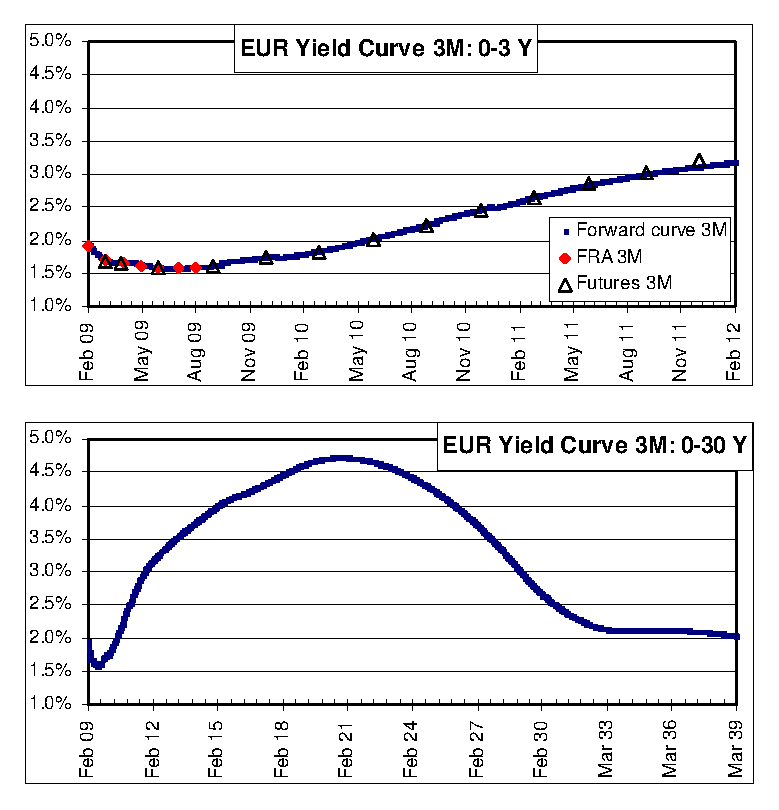
\includegraphics[scale=0.9]{./FigYC3M}
\caption{Yield curve on Euribor3M. Plots as in fig. \protect\ref{FigYC1M}. Cyan diamonds: quoted 3M FRAs. Green triangles: quoted 3M\ Futures.}
\label{FigYC3M}
\end{figure}

\begin{figure}[tbp]
\centering
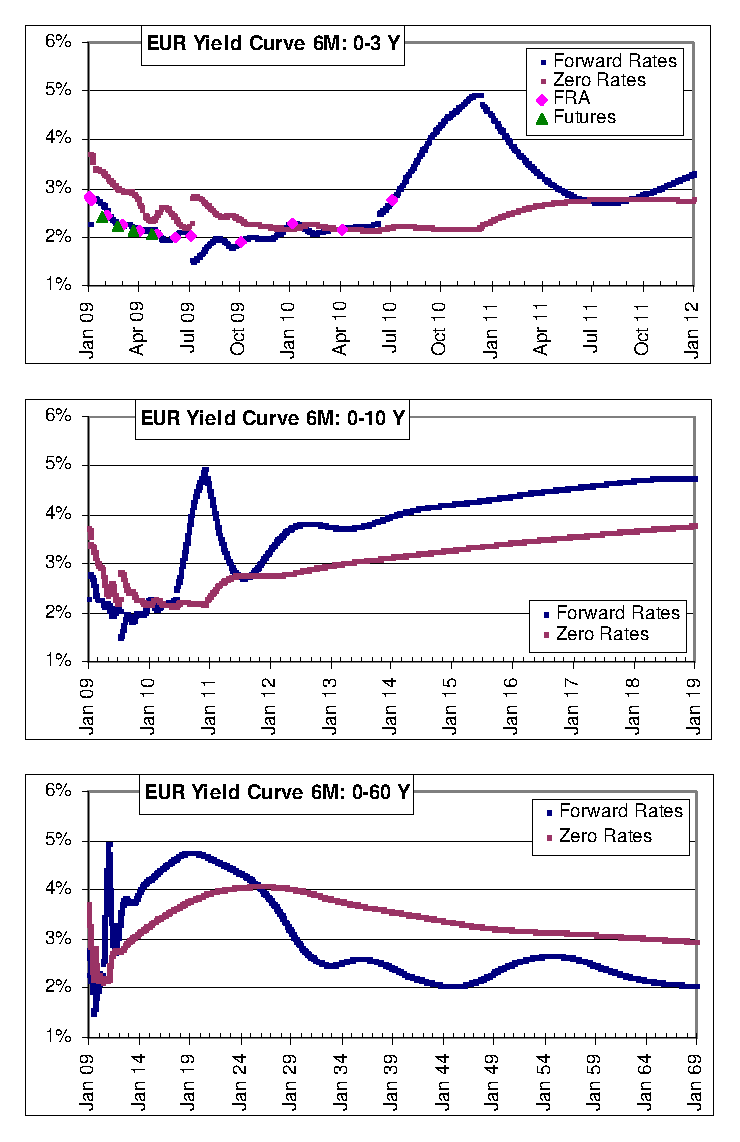
\includegraphics[scale=0.9]{./FigYC6M}
\caption{Yield curve on Euribor6M. Plots as in fig. \protect\ref{FigYC1M}. Cyan diamonds: quoted 6M FRAs. Green triangles: quoted 6M\ Futures.}
\label{FigYC6M}
\end{figure}

\begin{figure}[tbp]
\centering
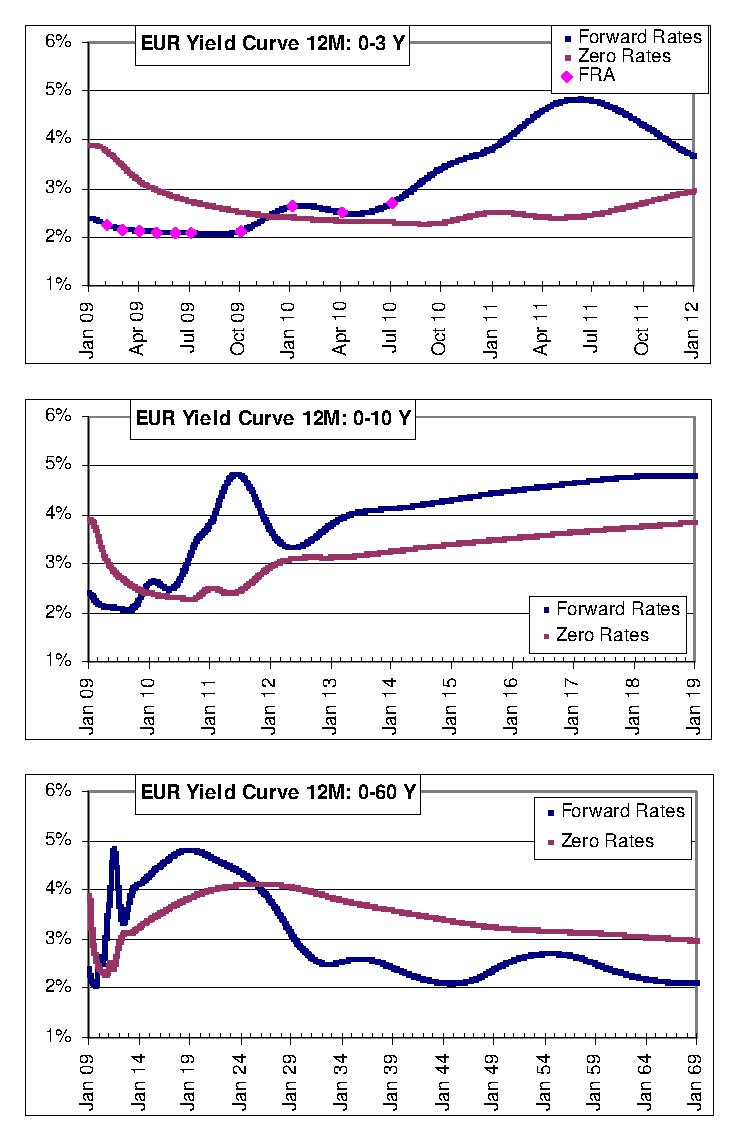
\includegraphics[scale=0.9]{./FigYC12M}
\caption{Yield curve on Euribor12M. Plots as in fig. \protect\ref{FigYC1M}. Cyan diamonds: quoted 12M FRAs.}
\label{FigYC12M}
\end{figure}

\section{\label{SecPricing2curves}Pricing Interest Rate Derivatives Using Separated Yield Curves for
Discounting and Forwarding}
In this section we revisit the general problem of pricing interest rate derivatives using two different yield curves for discounting and forwarding.
TBD, mettere solo cenni a quanto c'e' nell'altro paper.


\subsection{Quanto Adjustment}
TBD


\section{\label{SecConclusions}Conclusions}

TBD


\bibliographystyle{unsrt}
\bibliography{FinanceBibliography}

\end{document}
